\section{Experiments}
\label{sec:experiments}

\paragraph{Implementation Details}
Training used the ADAN optimizer with an initial learning rate of $1 \times 10^{-4}$, decayed to $0.02$. Sequences were resampled from 60 FPS to 30 FPS, yielding $S=150$ frames per five-second clip. Diffusion timesteps $T=1000$ were accelerated via DDIM with 50 sampling steps. SMPL axis-angle parameters were converted to 6D rotations using orthogonalization. Foot contact labels were derived from vertical foot/toe velocity near zero. All experiments trained on AIST++ break and middle hip-hop genres for testing, with the remaining eight genres for training. Multi-view 2D keypoints served as conditioning inputs. Batch size was fixed at 32 throughout.

\begin{figure}[htbp]
    \centering
    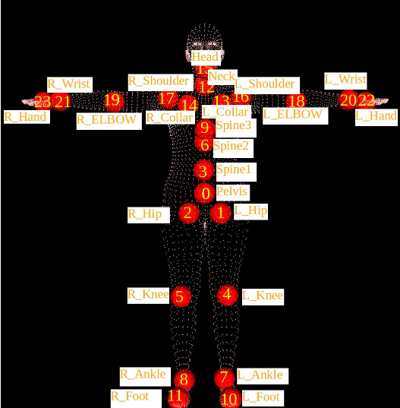
\includegraphics[width=0.5\textwidth]{Pictures/smpl.png}
    \caption{SMPL's 3D Joint Indicies Format (Tool used for Forward Kinematics in implementation)}
    \label{fig:smpl}
\end{figure}

\paragraph{Training Stability and Lambda Scheduling}
Early epochs set $\lambda_{\text{joints}}=0.01$, $\lambda_{\text{vel}}=1.0$, $\lambda_{\text{foot}}=0.1$. The velocity loss dominated, causing collapse to static poses where $\mathbf{R}_{t+1} \approx \mathbf{R}_t$. Direct matrix subtraction $\mathbf{R}_{t+1} - \mathbf{R}_t$ is not physically meaningful on $SO(3)$ and produced large gradients that overwhelmed the diffusion objective. The model learned that predicting no motion minimized loss.

To counteract collapse, lambda scheduling evolved: $\lambda_{\text{joints}}$ increased to $0.1$ by epoch 25, $\lambda_{\text{vel}}$ reduced to $0.01$ by epoch 40, and $\lambda_{\text{foot}}$ rose to $0.5$. Crucially, setting any auxiliary loss to zero caused immediate mean-pose collapse; all three losses required non-zero weights from initialization. The final stable configuration used $\lambda_{\text{joints}}=0.1$, $\lambda_{\text{vel}}=0.02$, $\lambda_{\text{foot}}=0.05$.

\paragraph{SNR Weighting Strategies}
Standard diffusion training with constant weighting $w_t=1$ yielded 32–36\% sample efficiency—most timesteps contributed negligible gradient after the SNR cliff. Experiments evaluated four strategies:
\begin{itemize}
    \item \textbf{Min-cap}: $w_t = \min(\text{SNR}_t, \gamma)$ with $\gamma=1$ created a steep cliff; 70\% of steps carried near-zero weight.
    \item \textbf{Decay min-cap}: Linear or sqrt decay schedules smoothed early steps but left the cliff intact.
    \item \textbf{Averaging}: $w_t = \frac{1}{2}[\min(\text{SNR}_t, 1) + \sqrt{1-t/T}]$ filled the dead zone, achieving ~50\% sample efficiency. This variant prevented collapse and maximized data utilization.
    \item \textbf{Normalization}: Per-batch normalization of $w_t$ stabilized training but slowed convergence when combined with high caps ($\gamma=2$).
\end{itemize}
The recommended setting used sqrt decay averaging with $\gamma=1$ and per-batch normalization disabled, doubling effective gradient flow compared to min-cap.

\begin{figure}[htbp]
\centering
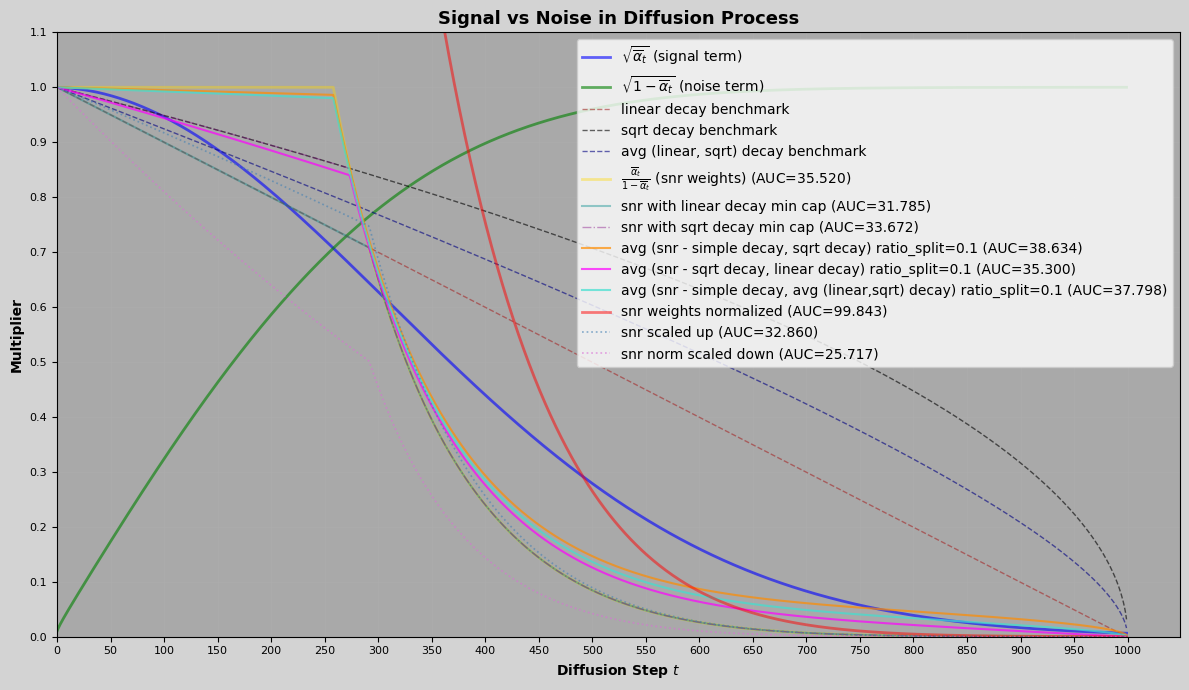
\includegraphics[width=\textwidth]{Pictures/snr.png}
\caption{Ablation of SNR weighting strategies for a $T=1000$ linear diffusion process ($\beta \in [1e-4, 0.02]$). Plotted are the signal term $\sqrt{\bar{\alpha}_t}$ and noise term $\sqrt{1-\bar{\alpha}_t}$, benchmark decay curves (linear, square root, and their average), and proposed SNR variants: simple ratio $\frac{\bar{\alpha}_t}{1-\bar{\alpha}_t}$, min-capped decays, ratio-split=0.1 blends, normalized, and scaled weights. Area-under-curve (AUC) percentages (cap=1.0) quantify integrated weight magnitude. Normalized SNR achieves the highest AUC (99.843\%), while simple SNR decays precipitously.}
\label{fig:snr}
\end{figure}

\paragraph{Temporal Modeling with PTSS}
Vectorized timesteps enable frame-wise noise schedules but risk combinatorial explosion. Probabilistic Timestep Sampling Strategy (PTSS) controls complexity. Experiments varied $p$, the probability of independent per-frame sampling:
\begin{itemize}
    \item $p=0.2$ to $0.5$ over epochs 1–50 showed steady loss decrease and growing prediction variance.
    \item $p>0.6$ introduced excessive variance, triggering SMPL forward kinematics violations in root position scale.
    \item Returning to $p=0.2$ after epoch 60 with learning rate increased to $2.5 \times 10^{-4}$ stabilized training.
\end{itemize}
PTSS improved beat alignment but required careful scheduling. Best practice: start with low $p$ and gradually increase, resetting to low $p$ if divergence occurs. Frame-independent timesteps offered no advantage over global timesteps for motion data; PTSS's primary benefit was preventing overfitting to a fixed schedule.

\paragraph{Model Architecture Ablations}
Two FiLM implementations were compared. Version~1 shared a single linear layer across all modulation points within a denoiser block. Version~2 used three separate linear layers for self-attention, cross-attention, and MLP outputs. Both applied identical parameters across frames.
\begin{itemize}
    \item Small models ($d=128$, $n_{\text{heads}}=4$) showed no performance gap.
    \item Large models ($d=256$, $n_{\text{heads}}=8$) revealed Version~2 converged marginally slower due to increased parameters.
    \item Version~1 was selected for production runs as parameter reduction mitigated overfitting on the 26k-sample dataset.
    \item The difference was negligible; architectural novelty lies in conditioning strategy, not FiLM multiplicity.
\end{itemize}

\paragraph{Convergence Monitoring and Target Metrics}
Tracking loss component magnitudes guided training:
\begin{itemize}
    \item $\mathcal{L}_{\text{joints}}$ target: 0.01–0.02. Below 0.01 indicated overfitting; above 0.03 required higher $\lambda_{\text{joints}}$.
    \item $\mathcal{L}_{\text{vel}}$ target: 0.05–0.10. Below 0.01 signaled static predictions; above 0.15 produced erratic motion.
    \item $\mathcal{L}_{\text{foot}}$ target: $10^{-4}$–$10^{-3}$. Above 0.01 revealed excessive foot sliding; below $10^{-4}$ over-constrained naturalness.
\end{itemize}
Prediction standard deviation steadily increased from near-zero to stable values around 0.1–0.2, confirming dynamic motion emergence. Final checkpoint achieved $\text{FID}_k=15.70$, $\text{Div}_k=4.85$, and beat-alignment score 0.239 on AIST++ test set, outperforming the MotionBERT baseline.
